
\documentclass{article}
\pdfpagewidth=8.5in
\pdfpageheight=11in
\usepackage{ijcai20}

% Use the postscript times font!
\usepackage{times}
\renewcommand*\ttdefault{txtt}
\usepackage{soul}
\usepackage{url}
\usepackage[hidelinks]{hyperref}
\usepackage[utf8]{inputenc}
\usepackage[small]{caption}
\usepackage{graphicx}
\usepackage{amsmath}
\usepackage{booktabs}
\usepackage{lipsum}
\urlstyle{same}

\usepackage[ruled,vlined,linesnumbered]{algorithm2e}
\usepackage{subcaption}
\usepackage{tikz}
\usepackage{pgfplots}
\usepgfplotslibrary{fillbetween}

% Layers
\pgfdeclarelayer{nodelayer}
\pgfdeclarelayer{edgelayer}
\pgfsetlayers{edgelayer,nodelayer,main}

% Node styles
\tikzstyle{box}=[fill=white, draw=black, shape=rectangle, minimum width=2cm, minimum height=0.5cm]
\tikzstyle{circle}=[fill=white, draw=black, shape=circle]

% Edge styles
\tikzstyle{directed edge double}=[<->]
\tikzstyle{directed edge}=[->]

% Plot size
\pgfplotsset{width=\textwidth/2.5,compat=newest} 


\let\OLDthebibliography\thebibliography
\renewcommand\thebibliography[1]{
  \OLDthebibliography{#1}
  \setlength{\parskip}{0pt}
  \setlength{\itemsep}{0pt plus 0.3ex}
}

\newcommand{\citationneeded}{\textsuperscript{[citation needed]}}
\newcommand\floor[1]{\lfloor#1\rfloor}
\newcommand\ceil[1]{\lceil#1\rceil}

\title{Message efficient Byzantine Reliable Broadcast protocols on known topologies}

\author{
Tim Anema$^1$\and
J{\'e}r{\'e}mie Decouchant$^1$
\affiliations
$^1$TU Delft\\
\emails
\{t.p.d.anema\}@student.tudelft.nl,
\{j.decouchant\}@tudelft.nl
}

\begin{document}

\maketitle

\begin{abstract}
\textbf{In this paper we consider the Reliable Communication and Byzantine Reliable Broadcast problems on partially connected networks with authenticated links. We consider the RC problem on partially connected networks, and the BRB problem on partially and fully connected networks. Danny Dolev's protocol works on the former, while Gabriel Bracha's \textit{authenticated double echo} protocol works on the latter in the case of a fully connected network. By layering the two protocols the BRB problem can be solved for partially connected networks.
The state-of-the-art protocols for these problems focus on unknown topologies, whereas we focus on known topologies. We show that these problems can be optimized when processes leverage this knowledge. Our simulations with our profiler show that we can drastically increase the message complexity and network usage (e.g., a reduction of XXX\% and XXX\% respectively with a 12B payload when N=150 and f=20 respectively) compared to naive with our optimizations and disjoint path solver.}

% The abstract should be short and give the overall idea:
% what is the background, the research questions, what is contribution, and what are the main conclusions.
% It should be readable as a stand-alone text (preferably no references to the paper or outside literature).
\end{abstract}

\section{Introduction}
\begin{itemize}
\item Introduce the topic and explain why it is important (motivation!).

\item Relate to the most relevant existing work from the literature (use BibTeX) \cite{example}, explain their contributions, and (critically) indicate what is still unanswered. 


\item Explain what the research questions for this work are. 
This usually is a subset of the unanswered questions. 

\item Summarize the main contributions/conclusions of this research.
NB: Make sure the title of the paper is a good match to the main research question / contribution / conclusion.

\item Briefly indicate how the rest of the paper fits together to answer the research question.
\end{itemize}

For a longer research paper, a section with more elaborate discussion of the literature may follow, but for short (conference) submissions, this is often included in the introduction.

\section{System model and problem statement}
\label{system-model}
% Choose one that fits your research best:
% \subsection{Methodology}
% Typically in general research articles, the second section contains a description of the research methodology, explaining what you, the researcher, is doing to answer the research question(s), and why you have chosen this method.
% For purely analytical work this is a description of the data collection or experimental setup on how to test the hypothesis, with a motivation.
% In any case this section includes references to necessary background information.

% \subsection{Formal Problem Description}
% For some types of work in computer science the methodology is standard: analyze the problem (e.g., make assumptions and derive properties), present a new algorithm and its theoretical background, proving its correctness, and evaluate unproven aspects in simulation.
% Then an explanation of the methodology is often omitted, and the setup of the evaluation is part of a later section on the evaluation of the ideas.\footnote{This already shows that there is no single outline to be given for all papers.}
% In this case, explain relevant concepts, theory and models in this section (with references) and relate them to your research question.
% Also this section then typically contains a more precise, formal description of the problem.

% Do not forget to give this section another name, for example after the problem you are solving.

Our model is defined by a set $\Delta=\{p_1, p_2,...,p_N\}$ of N processes, uniquely identified by an ID $i$ known to all others. In the Byzantine fault-model it is assumed that there are at most $f < \floor{N/3}$ Byzantine nodes, which can exhibit arbitrary behaviour. 

Furthermore, the processes are connected by a network which can be represented by an undirected graph $G=(V,E)$. In this graph every vertex represents a process $p_i$, such that $p_i \in \Delta$, which means $V=\Delta$ for all intents and purposes. It follows that the edges represent the communication links between nodes.
Processes $p_i, p_j \in \Delta$ have a direct communication link if there exists an edge $(v_i, v_j) \in E$, which they can use to directly communicate with each other. If there exists no such link, they will have to rely on other processes to relay their messages. We assume that these links are authenticated, i.e.\jd{,} messages delivered at $p_i \in \Delta$ via edge $(v_i, v_j) \in E$ are guaranteed to originate from $p_j$, and vice-versa. In addition to this, the links are reliable, i.e. messages will always arrive at $p_i$ if and only if $p_j$ sent them over edge $(v_i, v_j)$. However, there is no delivery time guarantee, so a link can be synchronous or asynchronous. Graph $G$ is known to all processes, and so are the IDs for every process. Furthermore, it is assumed the network is static, i.e. the network topology does not change, and the network lives for a considerable amount of time.

In order to send message data to others, processes can add information to the message header, which can be used to uniquely identify the message and add protocol specific information.

A Byzantine Reliable Broadcast (BRB) protocol guarantees the following properties:\\
(i) \textbf{Validity}: If process $p_i \in \Delta$ broadcasts message $m$, then every correct process $p_j \in \Delta$ delivers $m$ at some point.\\
(ii) \textbf{No duplication}: A message $m$ broadcast by process $p_i \in \Delta$ is not delivered more than once by every correct process $p_j \in \Delta$.\\
(iii) \textbf{Integrity}: If process $p_j \in \Delta$ delivers message $m$ with sender $p_i$, process $p_i$ has broadcast $m$ in the past.\\
(iv) \textbf{Agreement}: If process $p_i \in \Delta$ delivers message $m$, then $m$ will eventually be delivered by every correct process $p_j \in \Delta$.

% \begin{itemize}
%     \item \textbf{Validity}: If process $p_i \in \Delta$ broadcasts message $m$, then every correct process $p_j \in \Delta$ delivers $m$ at some point.
%     \item \textbf{No duplication}: A message $m$ broadcast by process $p_i \in \Delta$ is not delivered more than once by every correct process $p_j \in \Delta$.
%     \item \textbf{Integrity}: If process $p_j \in \Delta$ delivers message $m$ with sender $p_i$, process $p_i$ has broadcast $m$ in the past.
%     \item \textbf{Agreement}: If process $p_i \in \Delta$ delivers message $m$, then $m$ will eventually be delivered by every correct process $p_j \in \Delta$.
% \end{itemize}

We will be introducing improvements to both Dolev~\cite{dolev}, Bracha~\cite{bracha}, and Bracha-Dolev~\cite{bracha-dolev}, which make different assumptions about the network $G$ and the BRB guarantees. \jd{?}

\jd{why do you repeat the papers' assumptions here? Which assumptions do you make?}

Dolev assumes a network $G$ that is at least $2f+1$-connected, i.e. there are at least $2f+1$ vertex-disjoint paths from every vertex $v_i \in V$ to every vertex $v_j \in (V - \{v_i\})$. Furthermore, Dolev assumes Reliable Communication (RC) which guarantees the same properties as BRB, except for the agreement property. Bracha assumes a fully connected network $G$, i.e. for every pair $v_i,v_j \in V$ there exists an edge $(v_i, v_j) \in E$. Unlike Dolev, Bracha guarantees all BRB properties.

We make the same assumptions as the mentioned protocols, while adding topology knowledge and static long-lived networks.

\subsection*{Background}
In this section we will explain Dolev's and Bracha's protocols, and how they can be combined intro Bracha-Dolev.

\subsubsection{Dolev}
Dolev's protocol provides reliable communication when the network has authenticated links and is at least $2f+1$-connected.

When a message traverses the network, processes leverage the authenticated links to build a traversal path for each message. Said paths have two purposes: avoiding transmitting loops and message verification. 
The former is at play when processes relay messages to their neighbours; a message is forwarded to all neighbours, except to the transmitter and processes which are already present in the path. This is required in order to avoid messages circulating through the network indefinitely.
The paths are also used for verification; a message is delivered whenever it has been received over $f+1$ disjoint paths.

The basis for the correctness for Dolev's protocol lies in Menger's theorem~\cite{menger} which shows that there exist $2f+1$ disjoint paths between every pair of processes if a network is $2f+1$-connected, and the fact that at most $f$ of those paths can contain one or more Byzantine processes. This follows from the fact that a single process can only be in a single path, otherwise said path would not be disjoint, so the worst case is that all $f$ Byzantine processes are spread over all the $2f+1$ disjoint paths, which leaves $f+1$ paths not containing a Byzantine process.

There are multiple ways to implement the verification, but the problem is often reduced to a max flow problem or a minimum vertex cut problem. \jd{refs?} We will elaborate on the first option. In this case paths are modeled as a flow network where every edge has a capacity of one. The maximum flow through the network from source $p_j$ to sink $p_i$ is then equal to the amount of disjoint paths. The max flow can be found with the Ford-Fulkerson algorithm~\cite{ford_fulkerson} for example. \jd{this only works with non Byzantine processes}
Pseudocode for Dolev's protocol is provided in Algorithm~\ref{background:dolev}.

\begin{algorithm}
  \DontPrintSemicolon
  \SetKwFunction{DInit}{Init}
  \SetKwProg{Fn}{On event}{:}{}
  \Fn{\DInit}{
        delivered = False\;
        paths = $\emptyset$\;
  }
  
  \SetKwFunction{DRecv}{Receive}
  \Fn{\DRecv{$p_{recv}$, $m$, $path$}}{
        $path$ = $path \cup \{p_{recv}\}$\;
        \ForAll{$p_j \in neighbours - path$}{
            transmit($p_j$, $m$, $path$)\;
        }
  
        paths.add($path$)\;

        \uIf{paths contains $f+1$ node-disjoint paths to the origin \textbf{and} delivered = False}{
            deliver($m$)\;
            delivered = True\;
        }
  }
  
  \SetKwFunction{DBrd}{Broadcast}
  \Fn{\DBrd{$m$}}{
        deliver($m$)\;
        delivered = True\;
            
        \ForAll{$p_j \in neighbours$}{
            transmit($p_j$, $m$, $\emptyset$)\;
        }
  }
 \caption{Dolev's Reliable Communication algorithm}
 \label{background:dolev}
\end{algorithm}

\subsubsection{Bracha}
Unlike Dolev's protocol, Bracha's protocol requires a fully connected network while giving all BRB guarantees. \jd{is it not the case for Dolev? You haven't explained which BRB property is not satisfied by Dolev} The protocol has three phases: \textit{send}, \textit{echo}, and \textit{ready}.

When a process wants to broadcast a message it sends the payload in a \textit{send} message to all processes, including itself. When a process receives a \textit{send} messages, it responds by transmitting an \textit{echo} message to all processes with the corresponding content. Every process then waits for a quorum of \textit{echo} messages, which is $\ceil{\frac{N+f+1}{2}}$. 
After this quorum has been reached, or $f+1$ \textit{ready} messages have been received, a process will transmit its own \textit{ready} message to all processes. Finally, a message will be delivered when $2f+1$ corresponding \textit{ready} messages have been received, as can be seen in Algorithm~\ref{background:bracha}.

\begin{algorithm}[h]
  \DontPrintSemicolon
  \SetKwFunction{BInit}{Init}
  \SetKwProg{Fn}{On event}{:}{}
  \Fn{\BInit}{
        sentEcho = sentReady = delivered = False\;
        echos = readys = $\emptyset$\;
  }
  
  \SetKwFunction{BRecvEcho}{ReceiveEcho}
  \Fn{\BRecvEcho{$p_{recv}$, $m$}}{
        \uIf{\textbf{not} sentEcho}{
            \ForAll{$p_j \in neighbours$}{
                transmit($p_j$, $m$, ECHO)\;
            }
            
            sentEcho = True\;
        }
        
        echos.add($p_{recv}$)\;

        \uIf{len(echos) $\ge$ $\ceil{\frac{N+f+1}{2}}$ \textbf{and not} sentReady}{
            \ForAll{$p_j \in neighbours$}{
                transmit($p_j$, $m$, READY)\;
            }
            
            sentReady = True\;
        }
  }
  
  \SetKwFunction{BRecvReady}{ReceiveReady}
  \Fn{\BRecvReady{$p_{recv}$, $m$}}{
        readys.add($p_{recv}$)\;

        \uIf{len(readys) $\ge f+1$ \textbf{and not} sentReady}{
            \ForAll{$p_j \in neighbours$}{
                transmit($p_j$, $m$, READY)\;
            }
            
            sentReady = True\;
        }
        
        \uIf{len(readys) $\ge 2f+1$ \textbf{and not} delivered}{
            deliver($m$)\;
            delivered = True\;
        }
  }
  
  \SetKwFunction{BBrd}{Broadcast}
  \Fn{\BBrd{$m$}}{
        \ForAll{$p_j \in neighbours$}{
            transmit($p_j$, $m$, SEND)\;
            transmit($p_j$, $m$, ECHO)\;
        }
  }
 \caption{Bracha's authenticated double echo algorithm}
 \label{background:bracha}
\end{algorithm}

\subsubsection{Bracha-Dolev}
Dolev's and Bracha's protocol can be combined to achieve BRB guarantees in a multi-hop network, as described in \cite{bracha-dolev}. 

This works by layering the two protocols, where Dolev's protocol forms the bottom layer. This means that every Bracha broadcast is replaced by a Dolev broadcast, and every Bracha receive by a Dolev deliver. This process is shown in figure~\ref{background:bracha-dolev}.

By layering Bracha and Dolev, the latter emulates a fully connected network by enabling the former to reliably reach all processes. However, this means the message complexity of both protocols %, $\mathcal{O}(n^2)$ and $\mathcal{O}(n!)$ respectively,% 
is essentially multiplied.

Instead of simply layering the two protocols, a cross-layer version~\cite{bonomi2021practical} can be used which allows for greater optimization. For comparison, this version can be seen in figure~\ref{background:bracha-dolev}.

\begin{figure}
    \centering
    \begin{subfigure}{.2\textwidth}
      \centering
      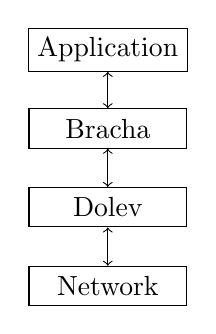
\begin{tikzpicture}
        	\begin{pgfonlayer}{nodelayer}
        		\node [style=box] (0) at (-4.25, 6.25) {Application};
        		\node [style=box] (1) at (-4.25, 5.25) {Bracha};
        		\node [style=box] (2) at (-4.25, 4.25) {Dolev};
        		\node [style=box] (3) at (-4.25, 3.25) {Network};
        	\end{pgfonlayer}
        	\begin{pgfonlayer}{edgelayer}
        		\draw [style=directed edge double] (0) to (1);
        		\draw [style=directed edge double] (1) to (2);
        		\draw [style=directed edge double] (2) to (3);
        	\end{pgfonlayer}
        \end{tikzpicture}
    %   \caption{Layering Bracha and Dolev forms the basis for Bracha-Dolev}
    \end{subfigure}
    \begin{subfigure}{.2\textwidth}
      \centering
      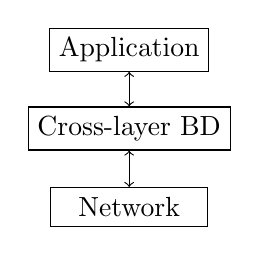
\begin{tikzpicture}
        	\begin{pgfonlayer}{nodelayer}
        		\node [style=box] (0) at (-4.25, 6.25) {Application};
        		\node [style=box] (1) at (-4.25, 5.25) {Cross-layer BD};
        		\node [style=box] (2) at (-4.25, 4.25) {Network};
        % 		\node [style=none] (3) at (-4.25, 3.25) {};
        	\end{pgfonlayer}
        	\begin{pgfonlayer}{edgelayer}
        		\draw [style=directed edge double] (0) to (1);
        		\draw [style=directed edge double] (1) to (2);
        	\end{pgfonlayer}
        \end{tikzpicture}
    %   \caption{A cross-layer combination can be used to improve performance~\cite{bonomi2021practical}}
    \end{subfigure}
    \caption{Bracha-Dolev can be implemented by simply layering the two protocols or by using a cross-layer protocol} %~\cite{bonomi2021practical}
    \label{background:bracha-dolev}
\end{figure}

\subsection*{Reducing the amount of messages}

While all mentioned protocols work well in their designed environments, there is naturally a substantial amount of redundant work.

In the case of Dolev, for example, the network is being flooded with the same message in order to reach all processes over at least $f+1$ vertex-disjoint paths. However, if the network is overprovisioned, i.e. the network is $k$-connected where $k > 2f+1$, the message will take more paths than strictly necessary. In addition to this, processes will send the message to (almost) all neighbours leading to overlapping paths. Even though recent improvements have reduced the amount of required messages 
%from $\mathcal{O}(n!)$ to nearly $\mathcal{O}(n)$~\cite{bonomi2019multihop}
, it is possible this can still be reduced if processes have knowledge of the network topology. The original paper describes a routed version which mitigates this problem. However, the actual creation of the routes is not discussed.

For Bracha there are similar inefficiencies. For example, Bracha uses all nodes to come to an agreement, while only a subset of size $\ceil{\frac{N+f+1}{2}} + f$ is needed in the \textit{echo} phase and a smaller subset of size $3f+1$ for the final \textit{ready} phase.

% The optimizations can be combined and applied to Bracha-Dolev, also reducing the amount of required messages for that protocol.

The aim of this paper is to reduce the amount of messages being transmitted and network usage even further, assuming that the processes know the network topology. In addition to this, it might be possible to improve the delivery complexity of Dolev in the process by taking advantage of the fact that messages will traverse fixed paths. Furthermore, while the general process for handling known topologies for Dolev has been described in the original paper~\cite{dolev}, no actual implementation has been provided, which is something this paper will also do and is an additional contribution of this work.


\section{Your contribution}
% In computer science typically the third section contains an exposition of the main ideas, for example the development of a theory, the analysis of the problem (some proofs), a new algorithm, and potentially some theoretical analysis of the properties of the algorithm.

% Do not forget to give this section another name, for example after the method or idea you are presenting.

% Some more detailed suggestions for typical types of contributions in computer science are described in the following subsections.

% \subsection*{Experimental work}
% In this case, this section will mostly contain a description of the methods/algorithms you will be comparing. Although not all methods need to be described in detail (providing appropriate references are available), make sure that you reveal sufficient details to a reader not familiar with these methods to: a) obtain a high-level understanding of the method and differences between them, and b) understand your explanation of the results.

% \subsection*{Improvement of an idea}
% In this case, you would need to explain in detail how the improvement works. If it is based on some observation that can be proven, this is a good place to provide that proof (e.g., of the correctness of your approach). 

\section{Evaluation}
\label{eval}
% As discussed earlier, in many sciences the methodology is explained in section 2 and this section only discusses the results. 
% However, in computer science, most often the details of the evaluation setup are described here first (simulation environment, etc.).
% Very important here is that any skilled reader would be able to reproduce this setup and then obtain the same results.

% Then, results are reported in an accessible manner through figures (preferably with captions that allow them to be understood without going through the whole text), observations are made that clearly follow from the presented results.
% Conclusions are drawn that follow logically from the previous material.
% Sometimes the conclusions are in fact hypotheses, which in turn may give rise to new experiments to be validated.

% You may want to give this section another name.

In this section we will discuss the methodology we used and the results of our optimizations.

\subsection{Methodology}
For our research we implemented an evaluation program in Go which uses goroutines~\cite{goroutines} as a process abstraction, and dedicated channels~\cite{channels} as communication links. The protocol instances are instantiated by the process wrappers, and they have access to a network and an application instance, which are defined by the interfaces containing \texttt{Send(dst, m)} and \texttt{Deliver(m)} respectively. The protocols themselves provide the \texttt{Init()}, \texttt{Receive(src, m)}, and \texttt{Broadcast(m)} functions.

In addition to the original protocols and improved version of Dolev~\cite{bonomi2019multihop} and a version of Dolev with naive routing was implemented. These two versions are the baseline for Dolev and Bracha-Dolev. 
%\textbf{TODO: discuss bonomi 10.}

We focus on message complexity and network consumption, which is defined by the total number of messages transmitted and total number of bytes transmitted, respectively. We mention latency when notable, but this is not a statistic we focus on. We define the latency as the time between the original broadcast and the final non-Byzantine node delivering the message. 

We use similar graphs as used in \cite{bonomi2021practical,bonomi2019multihop}: generalized wheels, multipartite wheels, and random regular graphs. For the tests we use an AMD Ryzen 5 2600 (3.4-3.9GHz) machine. The usage of channels leads to a different throughput per machine, but their performance will not limit the tests~\citationneeded and will not affect our main measurement.

We will run the tests with varying graphs, broadcasting process, byzantine processes, and parameters $N$, $k$, $f$, such that $N \ge 3f+1$ and $k \ge 2f+1$, and report the mean and standard deviation of five tests. In most tests a single process will broadcast a single message, unless the modifications being tested include \textbf{ORD.6} as it is specifically made for the case of multiple broadcasters.

\textbf{Remark}
Note that the latency will not be entirely representative of the latency in a real deployment, as our simulated links have low latency which means latency is largely influenced by computing time. 

\subsection{Impact of individual optimizations}
We evaluated the impact of individual optimizations on the message complexity and network consumption. Table~\ref{eval:individual-results} summarizes our findings for every individual modification compared to its baseline. The baseline is different for each protocol: for Dolev we compare to a version with naive routing, for Bracha we compare to the original version, and for Bracha-Dolev we compare to a version of Bracha-Dolev which uses naive routing for the Dolev layer and the original Bracha implementation. For these tests random graphs were used with a size of $N=150$ for Dolev and Bracha and $N=75$ for Bracha-Dolev, and we varied the $k$ and $f$ to find out when modifications are useful. 

We will illustrate some modifications with the aforementioned configuration.

There are several modification which perform well across the board, such as \textbf{ORD.1-3,7}, \textbf{ORB.1,2}, and \textbf{ORBD.1}. Others are slightly more nuanced however. For example, both \textbf{ORD.6} and \textbf{ORBD.2} perform better when the payload is large since they both rely on merging the payload, while adding slightly more information in a single header. 

Another optimization, \textbf{ORD.5}, does not show significant improvement. However, this lack of performance is offset by the fact that both \textbf{ORD.6} and \textbf{ORBD.2} rely on this modification. Another modification not showing significant improvements is \textbf{ORD.4}. While a part of this is likely caused by a non-optimal algorithm to reuse paths, it can also be attributed to the fact that I heavily relies on \textbf{ORD.3} to complete its task.

It is also interesting to note the dependencies between modifications. For example, \textbf{ORDB.2} on its own does not improve the protocol that much. However, when combined with \textbf{ORD.2} and \textbf{ORD.3} the amount of messages merged increases more than tenfold. The reason being that these two modifications cause a lot of messages to end up in the buffer and also cause quicker deliveries, leading to more merging in \textbf{ORDB.2}.

The opposite is also true, some modifications block the use of others. For example, \textbf{ORD.6} is unable to merge messages when \textbf{ORBD.2} is active, since they share the same buffer and \textbf{ORBD.2} changes the payload temporarily. For this reason, it is recommended to prefer \textbf{ORD.6} over \textbf{ORBD.2} when all processes are broadcasting identical payloads. 

\begin{table*}
  \centering
  \resizebox{\textwidth}{!}{
\begin{tabular}{c|cc|cc|cc|cc|}
\cline{2-9}
\textbf{}                         & \multicolumn{4}{c|}{\textbf{Small payload (12B)}}                                                  & \multicolumn{4}{c|}{\textbf{Large payload (12KB)}}                                                  \\ \hline
\multicolumn{1}{|c|}{\textbf{ID}} & \textbf{Msg. red. \%} & \textbf{Useful when} & \textbf{Usage red. \%} & \textbf{Useful when} & \textbf{Msg. red. \%} & \textbf{Useful when} & \textbf{Usage red. \%} & \textbf{Useful when} \\ \hline
\multicolumn{1}{|c|}{ORD.1}       & 10.18\% (2.65\%)            & small $k \wedge$ large $f$*               & 8.29\% (3.05\%)             & small $k \wedge$ large $f$*                & 8.67\% (3.47\%)            & small $k \wedge$ large $f$*               & 8.63\% (3.48\%)             & small $k \wedge$ large $f$*               \\ \hline
\multicolumn{1}{|c|}{ORD.2}       & 34.65\% (2.41\%)            & large $k$*               & 34.82\% (2.78\%)             & large $k$*               & 32.71\% (3.01\%)            & large $k$*               & 32.70\% (3.01\%)             & large $k$*               \\ \hline
\multicolumn{1}{|c|}{ORD.3}       & 63.06\% (1.37\%)            & always               & 10.11\% (2.94\%)             & always               & 62.03\% (1.77\%)            & always               & 61.29\% (1.80\%)             & always               \\ \hline
\multicolumn{1}{|c|}{ORD.4}       & 0.84\% (3.04\%)            & large $f$               & 0.77\% (3.46\%)             & large $f$               & -0.90\% (3.81\%)            & -               & -0.90\% (3.82\%)             & -               \\ \hline
\multicolumn{1}{|c|}{ORD.5}       & 2.09\% (2.99\%)            & always               & 1.63\% (3.43\%)             & always               & -0.06\% (4.04\%)            & -               & 0.07\% (4.05\%)             & -               \\ \hline
\multicolumn{1}{|c|}{ORD.6}       & 6.18\% (0.33\%)            & small $f$*               & 0.81\% (0.22\%)             & small $f$               & ?\% (?\%)            & TODO               & ?\% (?\%)             & TODO               \\ \hline
\multicolumn{1}{|c|}{ORD.7}       & 1.41\% (3.09\%)            & -               & 66.15\% (1.38\%)             & always               & ?\% (?\%)            & TODO               & ?\% (?\%)             & TODO               \\ \hline
\multicolumn{1}{|c|}{ORB.1}       & 0.41\% (0\%)            & always               & 0.41\% (0\%)             & always               & 0.41\% (0\%)            & always               & 0.41\% (0\%)             & always               \\ \hline
\multicolumn{1}{|c|}{ORB.2}       & 41.73\% (0\%)            & small $f$               & 41.73\% (0\%)             & small $f$               & 41.73\% (0\%)            & small $f$               & 40.91\% (0\%)             & small $f$               \\ \hline
\multicolumn{1}{|c|}{ORBD.1}      & 24.51\% (2.71\%)            & small $k \wedge$ small $f$*                & 24.68\% (2.73\%)             & small $k \wedge$ small $f$*                 & 21.66\% (2.03\%)            & small $k \wedge$ small $f$*                 & 21.66\% (2.03\%)             & small $k \wedge$ small $f$*                 \\ \hline
\multicolumn{1}{|c|}{ORBD.2}      & 1.25\% (1.12\%)            & always               & -3.04\% (1.96\%)             & never               & 0.2\% (0.82\%)            & -               & 0.14\% (0.83\%)             & -               \\ \hline
\end{tabular}
    }
  \caption{Effect of modifications measured on random graphs compared to their respective protocol standard. The mean reduction and according standard error is listed, in addition to a small description of the best use-cases. Note that descriptions marked with a star* are always useful, but will perform best in the given use-case.}
  \label{eval:individual-results}
\end{table*}

% \begin{table}[]
% \begin{tabular}{ll|ll|ll|ll|ll|}
% \cline{3-10}
% \multicolumn{1}{c}{\textbf{}}     & \multicolumn{1}{c|}{\textbf{}} & \multicolumn{4}{c|}{\textbf{Small payload}}                                                  & \multicolumn{4}{c|}{\textbf{Large payload}}                                                                       \\ \hline
% \multicolumn{1}{|l|}{\textbf{ID}} & \textbf{Protocol}              & \textbf{Msg. red. \%} & \textbf{Useful when} & \textbf{Usage red. \%} & \textbf{Useful when} & \multicolumn{1}{l|}{\textbf{Msg. red. \%}} & \textbf{Useful when} & \textbf{Usage red. \%} & \textbf{Useful when} \\ \hline
% \multicolumn{1}{|l|}{}            &                                &                       &                      &                        &                      &                                            &                      &                        &                      \\ \cline{1-2}
% \multicolumn{1}{|l|}{}            &                                &                       &                      &                        &                      &                                            &                      &                        &                      \\ \cline{1-2}
% \multicolumn{1}{|l|}{}            &                                &                       &                      &                        &                      &                                            &                      &                        &                      \\ \cline{1-2}
% \multicolumn{1}{|l|}{}            &                                &                       &                      &                        &                      &                                            &                      &                        &                      \\ \cline{1-2}
% \multicolumn{1}{|l|}{}            &                                &                       &                      &                        &                      &                                            &                      &                        &                      \\ \cline{1-2}
% \multicolumn{1}{|l|}{}            &                                &                       &                      &                        &                      &                                            &                      &                        &                      \\ \cline{1-2}
% \multicolumn{1}{|l|}{}            &                                &                       &                      &                        &                      &                                            &                      &                        &                      \\ \cline{1-2}
% \multicolumn{1}{|l|}{}            &                                &                       &                      &                        &                      &                                            &                      &                        &                      \\ \cline{1-2}
% \multicolumn{1}{|l|}{}            &                                &                       &                      &                        &                      &                                            &                      &                        &                      \\ \hline
% \end{tabular}
% \end{table}

\subsection{Improvements}
In addition to comparing individual modification we will also compare our full protocol in the case of Dolev and Bracha-Dolev. Figure~\ref{eval:overal-reduction} shows the reduction of our protocol compared to Dolev, Bracha and Bracha-Dolev with regards to the message complexity. The reduction is relative to the same baseline used for the individual modifications.

For Dolev and Bracha-Dolev we again use random graphs with $N=150$ and $N=75$ respectively, and vary the connectivity $k$. The number of Byzantine nodes $f$ is defined by $\floor{\frac{k-1}{2}}$. In the case of Bracha we have can only use fully connected graphs, and will therefore vary the number of processes $N$ depending on the connectivity. The number of byzantine nodes in this case is defined by $\floor{\frac{k}{4}}$. In all cases the payload size is equal to 12B. 

These tests show we are able to achieve a mean reduction of 79.49\% (+-0.93\%) for Dolev, 23.32\% for Bracha and 89.54\% (+-0.22\%) for Bracha-Dolev under the conditions mentioned above. The reduction in bytes transmitted is similar: 85.86\% (+-0.68\%), 23.32\%, and 92.32\% (+-0.17\%) respectively. 

\begin{figure}[h]
    \centering
    
    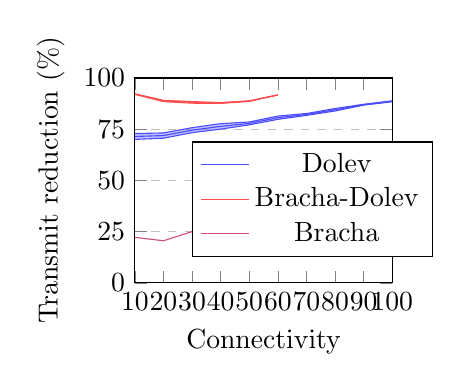
\begin{tikzpicture}
        \begin{axis}[
            xlabel={Connectivity},
            ylabel={Transmit reduction (\%)},
            xmin=10, xmax=100,
            ymin=0, ymax=100,
            xtick={10,20,30,40,50,60,70,80,90,100},
            ytick={0,25,50,75,100},
            legend style={at={(0.69,0.69)},
	        anchor=north,legend columns=1},
            ymajorgrids=true,
            grid style=dashed,
        ]
        
        \addplot[
            color=blue!70,
            ]
            coordinates {
            (10,71.44)(20,71.89)(30,74.52)(40,76.38)(50,77.82)(60,80.61)(70,82.19)(80,84.49)(90,86.92)(100,88.62)
            };
        \addlegendentry{Dolev}
        
        \addplot[
            color=red!70,
            ]
            coordinates {
            (10,92.14)(20,88.80)(30,88.08)(40,87.79)(50,88.72)(60,91.72)
            };
        \addlegendentry{Bracha-Dolev}
        
        \addplot[
            color=purple!70,
            ]
            coordinates {
            (10,22.22)(20,20.54)(30,25.02)(40,22.57)(50,24.73)(60,19.63)(70,22.67)(80,21.71)(90,27.13)(100,26.99)
            };
        \addlegendentry{Bracha}
        
        \addplot[
            name path=dolev_up,
            color=blue!70,
            ]
            coordinates {
            (10,72.86)(20,73.17)(30,75.74)(40,77.72)(50,78.52)(60,81.42)(70,82.65)(80,85.09)(90,87.17)(100,88.86)
            };
        \addplot[
            name path=dolev_down,
            color=blue!70,
            ]
            coordinates {
            (10,70.02)(20,70.61)(30,73.30)(40,75.04)(50,77.12)(60,79.80)(70,81.73)(80,83.89)(90,86.76)(100,88.39)
            };
        \addplot[blue!50,fill opacity=0.5] fill between[of=dolev_up and dolev_down];
        
        \addplot[
            name path=bdolev_up,
            color=red!70,
            ]
            coordinates {
            (10,92.26)(20,89.11)(30,88.47)(40,87.99)(50,88.85)(60,91.72)
            };
        \addplot[
            name path=bdolev_down,
            color=red!70,
            ]
            coordinates {
            (10,92.02)(20,88.49)(30,87.70)(40,87.59)(50,88.60)(60,91.72)
            };
        \addplot[red!50,fill opacity=0.5] fill between[of=bdolev_up and bdolev_down];
        \end{axis}
        \end{tikzpicture}
    \caption{Reduction  of message complexity using K-random graphs and fully-connected graphs (Bracha), while varying the connectivity.}
    \label{eval:overal-reduction}
\end{figure}

\subsection{Scalability}
In real deployments the number of processes in the network will likely scale quickly, which is why we also evaluated the scalability of the protocol for an increasing number of processes. We considered graphs which include 25 to 150 processes in increments of 25. The connectivity $k$ and Byzantine parameter $f$ are defined as $k=\floor{\frac{N}{3}}$ and $f=\floor{\frac{k-1}{2}}$ for (Bracha-)Dolev and $f=\floor{\frac{k}{4}}$ for Bracha. The other configuration is identical to the previous sections.

The evaluation for Bracha-Dolev was unable to continue after 75 processes, due to resource contraints; the version with naive routing an no additional optimizations was using too much memory\footnote{12GiB on a 16GiB system in this case} during testing. 
%Our optimized version had no issue reaching the final tests, but it was also using a considerable amount of memory in the process. 
We expect the trend of outperforming the base version on larger networks to continue, leading us to believe the reduction would be around 87\% for the larger networks.

From these experiments we can see that the message complexity is not decreasing, which means in terms of message complexity and network usage our modified versions scale well with the number of processes. However, the latency is still doubling after each increment, suggesting exponential growth. The modified protocols still outperformed the baseline in term of latency by 25.16\%, 22.38\%, and 50.19\% for Dolev, Bracha, and Bracha-Dolev respectively.

\begin{figure}[h]
    \centering
    
    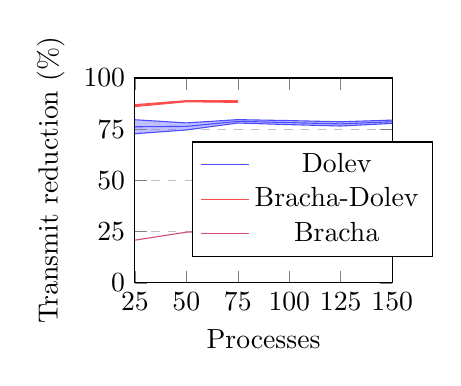
\begin{tikzpicture}
        \begin{axis}[
            xlabel={Processes},
            ylabel={Transmit reduction (\%)},
            xmin=25, xmax=150,
            ymin=0, ymax=100,
            xtick={25,50,75,100,125,150},
            ytick={0,25,50,75,100},
            legend style={at={(0.69,0.69)},
	        anchor=north,legend columns=1},
	        ymajorgrids=true,
            grid style=dashed,
        ]
        
        \addplot[
            color=blue!70,
            ]
            coordinates {
            (25,76.20)(50,76.36)(75,78.85)(100,78.21)(125,77.59)(150,78.63)
            };
        \addlegendentry{Dolev}
        \addplot[
            color=red!70,
            ]
            coordinates {
            (25,86.51)(50,88.67)(75,88.49)
            };
        \addlegendentry{Bracha-Dolev}
        \addplot[
            color=purple!70,
            ]
            coordinates {
            (25,20.83)(50,24.73)(75,25.88)(100,23.76)(125,19.79)(150,25.27)
            };
        \addlegendentry{Bracha}
        
        \addplot[
            name path=dolev_up,
            color=blue!70,
            ]
            coordinates {
            (25,79.62)(50,78.07)(75,79.67)(100,79.20)(125,78.62)(150,79.44)
            };
        \addplot[
            name path=dolev_down,
            color=blue!70,
            ]
            coordinates {
            (25,72.79)(50,74.64)(75,78.02)(100,77.23)(125,76.56)(150,77.83)
            };
        \addplot[blue!50,fill opacity=0.5] fill between[of=dolev_up and dolev_down];
        \addplot[
            name path=bdolev_up,
            color=red!70,
            ]
            coordinates {
            (25,86.98)(50,88.93)(75,88.88)
            };
        \addplot[
            name path=bdolev_down,
            color=red!70,
            ]
            coordinates {
            (25,86.05)(50,88.40)(75,88.10)
            };
        \addplot[red!50,fill opacity=0.5] fill between[of=bdolev_up and bdolev_down];
        \end{axis}
        \end{tikzpicture}
    \caption{Reduction of message complexity using K-random graphs and fully-connected graphs (Bracha), while varying the number of processes.}
\end{figure}

\subsection{Discussion}
% Results can be compared to known results and placed in a broader context.
% Provide a reflection on what has been concluded and how this was done.
% Then give a further possible explanation of results.

% You may give this section another name, or merge it with the one before or the one hereafter.
While our results are promising, we have focused on two main statistics: message complexity and network usage. This means that other statistics such as latency have sometimes been sacrificed in order to enhance our chosen statistics, as is the case with \textbf{ORD.6} and \textbf{ORBD.2} for example. This might not be desired in some systems.

As mentioned earlier, the measured latency is not fully representative of the real world. Something similar is true for the measured network usage, as we use size of internal structures as measurement. While this size is mostly representative of the actual size, it also includes some internal headers which would not be transmitted, and should therefore not be included. However, this will have no significant impact on our results as all measurements will include a similar size for internal data, which means the relative reductions will not be affected.

We can safely conclude that we can indeed reduce the number of messages when leveraging topology knowledge, but the system model might be too strict for modern networks as they are generally dynamic instead of static. 

\section{Broader impact and reproducibility}
\label{broader-impact}
% Reflect on the ethical aspects of your research and discuss the reproducibility of your methods.
% In this section we will briefly discuss the broader impact of our modifications to the BRB protocols handled in our paper, and we will also make note of the reproducibility of our evaluation.

Our research focused on improving existing protocols. This means we guarantee the same properties as the original protocols, while putting the network under less stress in certain systems. For this reason, there are no inherit risks to our work. In addition to this, there are limited malicious uses for our work, as it works as an underlying protocol similar to the regular internet protocol. 
However, our modifications add a considerable amount of complexity to the protocol, allowing for more developer error possibly leading to violated protocol properties.

% Depending on how the protocols are applied, our work could reduce network and system usage. This leads to either a higher capacity of the broadcast layer or a reduced energy footprint of the system. The latter always has positive impact, while the former can be negative if the system in question in malicious.

Now that we have discussed the broader impact of our work, its reproducibility should also be mentioned. All of our results are retrieved from a standalone binary whose source will be published together with this paper. The program has a low barrier of entry and can be used by anyone, since the program is written in widely supported language (Go) and has no other system dependencies. The program can be found in the GitLab repository\footnote{TODO: link}.

% The exact configurations used can be deduced from the evaluation section, and these can then be executed by the program. The exact graphs used for evaluation will also be published along with the code, although a user can also choose to generate new graphs. 

It is important to note that results may be different for every computer, as the program will execute everything as fast as possible. However, the relative differences between the original protocols and our improved versions will be closer to the results showed in our paper.

% To conclude, we believe our research does not have significant negative impact. Furthermore, everyone should be able to run our evaluation program themselves and verify our results. If desired, one can also implement our optimizations in another language using the descriptions and pseudocode we provided.

% \input{sections/discussion}

\section{Conclusions and Future Work}
Summarize the research question(s) and the answers to the research question(s).
Make statements.
Highlight interesting elements.

Discuss open issues, possible improvements, and new questions that arise from this work; formulate recommendations for further research.

ideally, this section can stand on its own: it should be readable without having read the earlier sections.

\bibliographystyle{IEEEtran}
\bibliography{references}

\appendix
\section{Appendix}
% \section{The obvious}
% \subsection{Reference use}
% \begin{itemize}
% \item use a system for generating the bibliographic information automatically from your database, e.g., use BibTex and/or Mendeley, EndNote, Papers, or \ldots
% \item all ideas, fragments, figures and data that have been quoted from other work have correct references
% \item literal quotations have quotation marks and page numbers
% \item paraphrases are not too close to the original
% \item the references and bibliography meet the requirements
% \item every reference in the text corresponds to an item in the bibliography and vice versa
% \end{itemize}

% \subsection{Structure}
% Paragraphs
% \begin{itemize}
% \item are well-constructed
% \item are not too long: each paragraph discusses one topic
% \item start with clear topic sentences
% \item are divided into a clear paragraph structure
% \item there is a clear line of argumentation from research question to conclusions
% \item scientific literature is reviewed critically
% \end{itemize}

% \subsection{Style}
% \begin{itemize}
% \item correct use of English: understandable, no spelling errors, acceptable grammar, no lexical mistakes 
% \item the style used is objective
% \item clarity: sentences are not too complicated (not too long), there is no ambiguity
% \item attractiveness: sentence length is varied, active voice and passive voice are mixed
% \end{itemize}

% \subsection{Tables and figures}
% \begin{itemize}
% \item all have a number and a caption
% \item all are referred to at least once in the text
% \item if copied, they contain a reference
% \item can be interpreted on their own (e.g. by means of a legend)
% \end{itemize}

\subsection{Pseudocode}
\label{appendix-pseudocode}
\begin{algorithm}
  \DontPrintSemicolon
  \SetKwFunction{DInit}{Init}
  \SetKwProg{Fn}{On event}{:}{}
  \Fn{\DInit}{
        delivered = False\;
        paths = $\emptyset$\;
  }
  
  \SetKwFunction{DRecv}{Receive}
  \Fn{\DRecv{$p_{recv}$, $m$, $path$, $planned$}}{
        $path$ = $path \cup \{p_{recv}\}$\;
        \ForAll{$p_j \in planned$}{
            transmit($p_j$, $m$, $path$, $planned$)\;
        }
  
        paths.add($path$)\;

        \uIf{paths contains $f+1$ node-disjoint paths to the origin \textbf{and} delivered = False}{
            deliver($m$)\;
            delivered = True\;
        }
  }
  
  \SetKwFunction{DBrd}{Broadcast}
  \Fn{\DBrd{$m$}}{
        deliver($m$)\;
        delivered = True\;
            
        \ForAll{$(p_j, route) \in routingTable$}{
            transmit($p_j$, $m$, $\emptyset$, $route$)\;
        }
  }
 \caption{Dolev's Reliable Communication routed algorithm}
 \label{background:dolev}
\end{algorithm}

\begin{algorithm}[h]
  \DontPrintSemicolon
  \SetKwFunction{BInit}{Init}
  \SetKwProg{Fn}{On event}{:}{}
  \Fn{\BInit}{
        sentEcho = sentReady = delivered = False\;
        echos = readys = $\emptyset$\;
  }
  
  \SetKwFunction{BRecvEcho}{ReceiveEcho}
  \Fn{\BRecvEcho{$p_{recv}$, $m$}}{
        \uIf{\textbf{not} sentEcho}{
            \ForAll{$p_j \in neighbours$}{
                transmit($p_j$, $m$, ECHO)\;
            }
            
            sentEcho = True\;
        }
        
        echos.add($p_{recv}$)\;

        \uIf{len(echos) $\ge$ $\ceil{\frac{N+f+1}{2}}$ \textbf{and not} sentReady}{
            \ForAll{$p_j \in neighbours$}{
                transmit($p_j$, $m$, READY)\;
            }
            
            sentReady = True\;
        }
  }
  
  \SetKwFunction{BRecvReady}{ReceiveReady}
  \Fn{\BRecvReady{$p_{recv}$, $m$}}{
        readys.add($p_{recv}$)\;

        \uIf{len(readys) $\ge f+1$ \textbf{and not} sentReady}{
            \ForAll{$p_j \in neighbours$}{
                transmit($p_j$, $m$, READY)\;
            }
            
            sentReady = True\;
        }
        
        \uIf{len(readys) $\ge 2f+1$ \textbf{and not} delivered}{
            deliver($m$)\;
            delivered = True\;
        }
  }
  
  \SetKwFunction{BBrd}{Broadcast}
  \Fn{\BBrd{$m$}}{
        \ForAll{$p_j \in neighbours$}{
            transmit($p_j$, $m$, SEND)\;
            transmit($p_j$, $m$, ECHO)\;
        }
  }
 \caption{Bracha's authenticated double echo algorithm}
 \label{background:bracha}
\end{algorithm}



\end{document}

